\chapter{Historie \legoM}

Historie firmy \lego{ }je velmi dlouhá a sahá až do roku 1932~\cite{lego_GroupHistory1930s} a prakticky to samé lze říct o stavebnici \legoM, jejíž počátky se datují k roku 1998~\cite{lego_mindstormsHistory} (období, kdy již počítač začínali mívat běžní lidé doma).

% TODO: kapitola LEGO TECHNIC

\section{\legoM{ }RCX}

První verze byla označena jako \legoM{ }RCX\footnote{RCX = Robotic Command eXplorers} Intelligent Brick and Robotics Invention System a  obsahovala 8-bitový mikrokontrolér Hitachi H8/3292~\cite{hitachi_microcontrolerH8series} s procesorem H8/300 taktovaným na 16~MHz a~s~32~KB~RAM~\cite{legoMindstormsRCX_Manual}.

\begin{figure}[h]
	\centering
	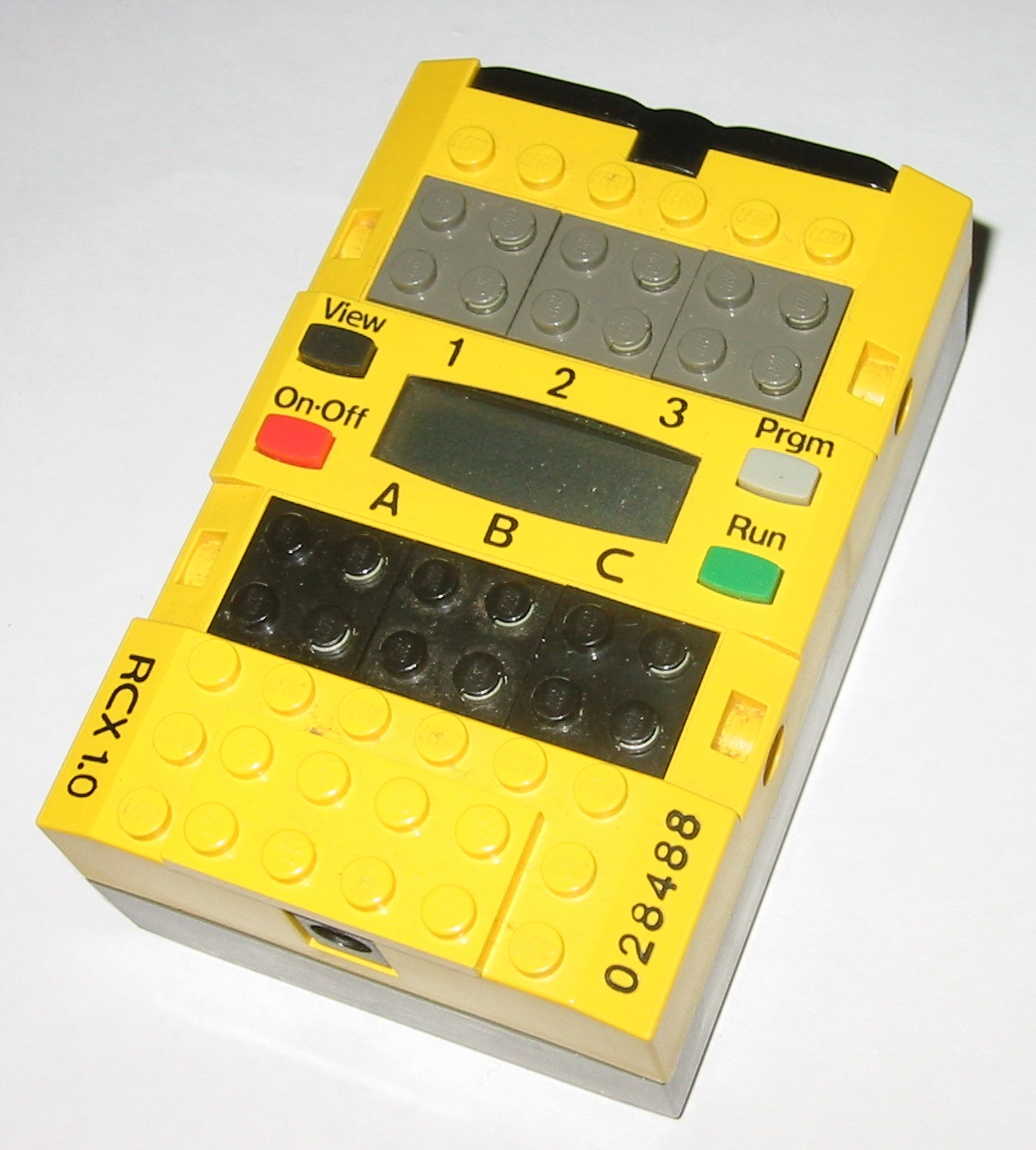
\includegraphics[width=250px]{images/lego-mindstorms-rcx_wikipedia.jpg}
	\caption[\legoM{ }RCX]{\legoM{ }RCX\protect\footnotemark}
	\label{fig:lego-mindstorms-rcx-wikipedia}
\end{figure}

\footnotetext{Zdroj: \url{https://en.wikipedia.org/wiki/Lego_Mindstorms}} 

Oficiálně bylo možné stavebnici programovat ve dvou prostředích. První prostředí ROBOLAB, založené na programu \labview{ }od firmy \NI, bylo pro výukové účely (do škol) a bylo součástí výukového setu. 
Běžní zákazníci (lidé, kteří si kupovali stavebnici domů) měli k dispozici RCX Code, které bylo jednodušší na obsluhu a používání, ale nemělo tak rozsáhle možnosti programování. 
Zároveň vznikly i vývojové prostředí třetích stran, které umožňovali programování v mnoha běžně používaných jazycích (C++, Java, \dots).

Již v prvním roce prodeje stavebnice vznikla soutěž {\it FIRST} LEGO League (FLL)\footnote{{\it FIRST} = For Inspiration and Recognition of Science and Technology}. 
Cílem soutěže je povzbudit a motivovat k navrhování, stavění a programování vlastních inteligentních systémů~\cite{lego_FLL-about}. 
Jednotlivá kola probíhají po celém světě a lze postoupit až do celosvětového finále. % TODO: FLL - ověřit možnost postupu do celosvětového finále
Účastníci musí být ve věku od 10 do 16 let. 


\section{\legoM{ }NXT}

Následující verzi vydalo \lego{ }v roce 2006~\cite{lego_mindstormsHistory}. 
Byl kompletně změněn způsob připojování jednotlivých modulů. 
Moduly se již nepřipojují pomocí speciálních \lego{ }kostek, ale využívají upravený konektor RJ-12 % TODO: upravený konektor -> méně běžnou variantu konektoru RJ-12
(kolík sloužící pro správné zapojení konektoru, je oproti běžné telefonní RJ-12, umístěn mimo střed~\cite{legoMindstorms_rj12-connector}). % -- na pravou stranu z pohledu od kabelu 

\begin{figure}[h]
	\centering
	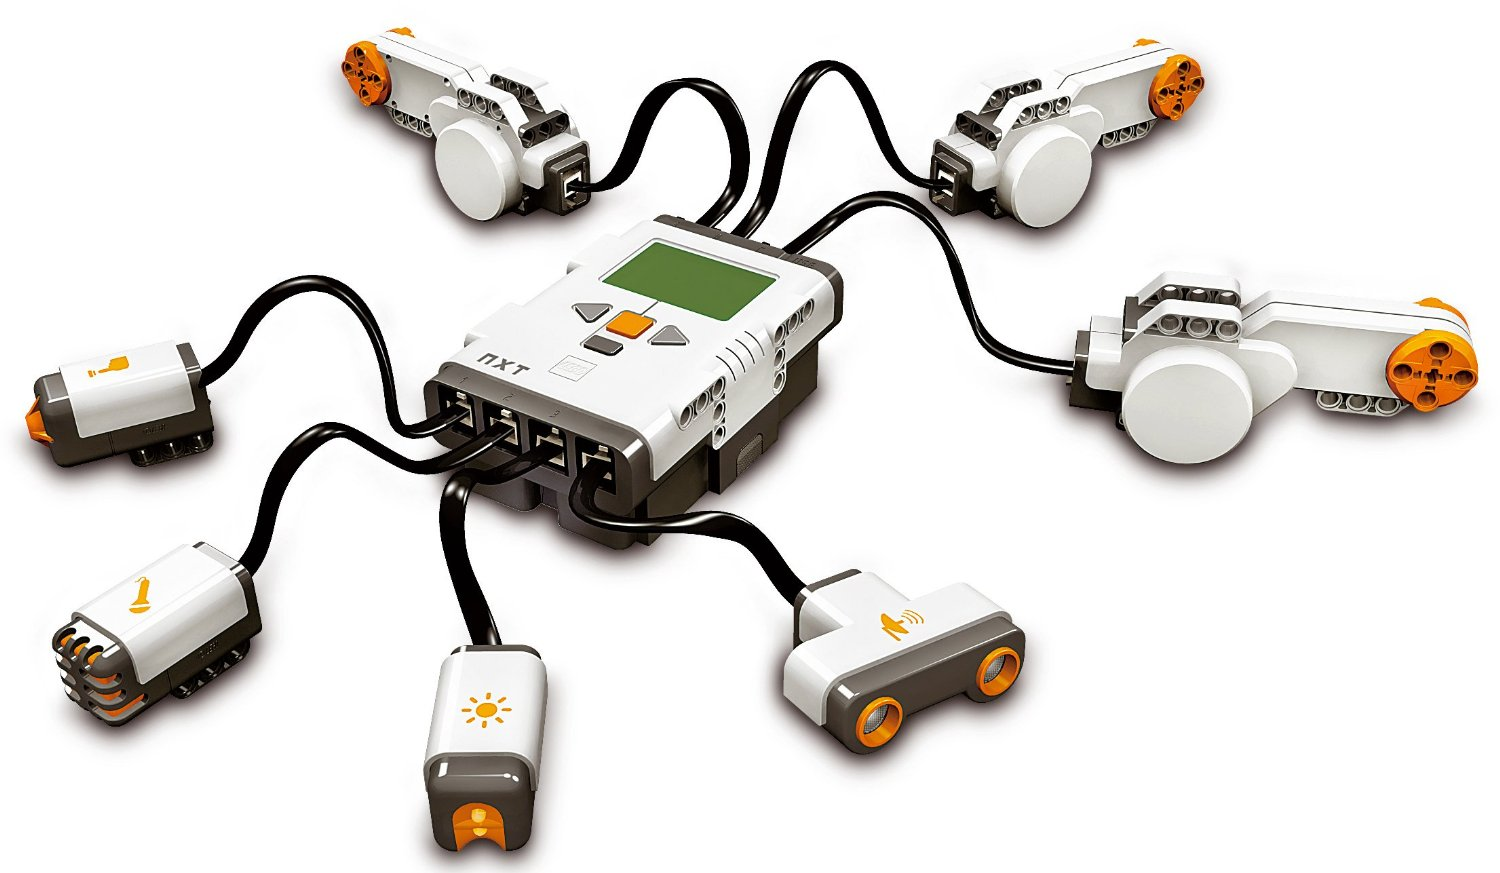
\includegraphics[width=\textwidth]{images/lego-mindstorms-nxt_with-modules.jpg}
	\caption[\legoNXT{ }s komponenty, které lze používat]{\legoNXT{ }s komponenty, které lze používat\protect\footnotemark}
	\label{fig:lego-mindstorms-nxt_with-modules}
\end{figure}

Řídící kostka (dále jen \brick{}) % TODO: formátování speciálních výrazů
se již neprogramuje přes infraport, ale využívá se standardní USB kabel, případně integrovaný Bluetooth~\cite{legoMindstormsNXT_hardware}.

Po hardwarové stránce došlo ke značnému posunu. Původní 8-bitový mikrokontrolér byl nahrazen 32-bitovým ARM mikrokontrolérem % TODO: mikrokontrolér/mikroprocesor/procesor
 AT91SAM7S256 (256~KB~FLASH, 64~KB~RAM, 48~MHz) a k němu byl přidán 8-bitový ko-procesor ATmega48 (4~KB~FLASH, 512~Byte~RAM, 8~MHz). 
Oba tyto procesory dodávala firma Atmel (nyní již Microchip)~\cite{legoMindstormsNXT_hardware}.

\footnotetext{Zdroj: \url{http://www.itnetwork.cz/java/lego-nxt/seznameni-s-nxj-pro-lego-nxt}} 

\brick{ }lze programovat pomocí vývojového prostředí NXT-G\footnote{NXT-G = NXT Graphic - grafické} (viz obrázek \ref{fig:lego-mindstorms-nxt-g}), které \lego{ }vyvinulo opět ve spolupráci s  \NI{~}\cite{legoMindstormsNXT_NXT-G}. 
Zároveň \NI{ }dodává toolbox do \labview{ }ve kterém lze \brick{ }také programovat. 

\legoNXT{ }má ovšem bohatou nabídku alternativních programovacích prostředí, které lze využít k vytváření kódu pro \brick. 
Některé fungovali již na RCX a byly upraveny i pro NXT. 
Jako příklad mohu uvést jedno z nejpoužívanějších prostředí BricxCC\footnote{BricxCC = Bricx Command Center} s jazykem NXC\footnote{NCX = Not eXactly C}. 
NCX je vysokoúrovňový open-source jazyk podobný C~\cite{legoWikipediaNXT_NXC}.

\begin{figure}[h]
	\centering
	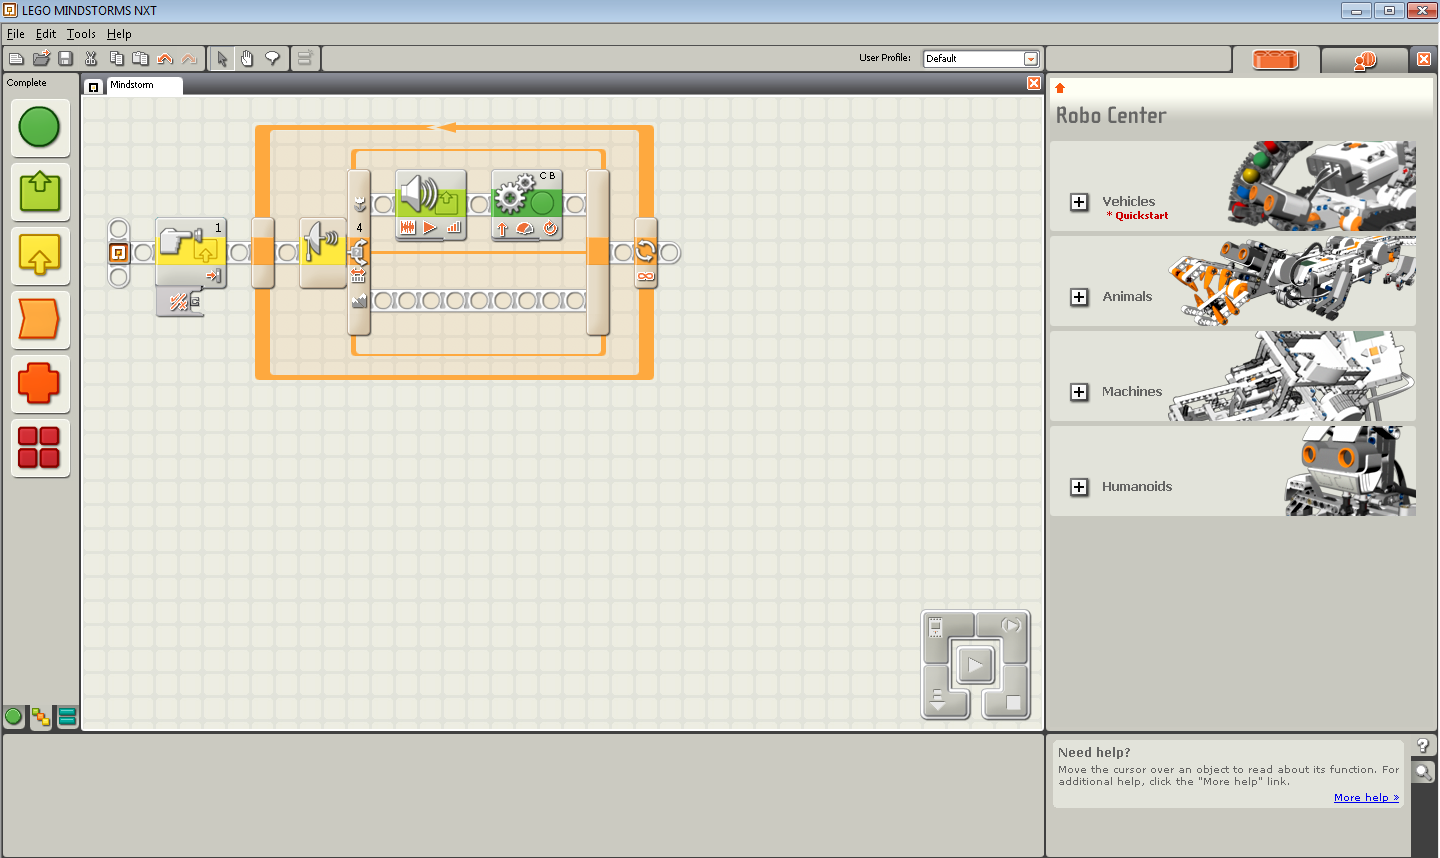
\includegraphics[width=\textwidth]{images/lego-mindstorms-nxt-g.png}
	\caption[\legoNXT{-G}]{\legoNXT{-G}\protect\footnotemark}
	\label{fig:lego-mindstorms-nxt-g}
\end{figure}

\footnotetext{Zdroj: \url{http://lukedainton-robots.blogspot.cz/2012/07/control-systems-shooterbot-nxt-g.html}} 
Existují ale i komerční varianty. 
Například ROBOTC~\cite{legoProgramingPlatform_ROBOTC} je univerzální programovací prostředí a jazyk umožňující programovat větší množství hardwaru (od \legoM{ }RCX, NXT, EV3 až po Arduino nebo PIC). 
Jak již název napovídá, ROBOTC je založen na jazyku C (ANSI-C).
Uživatel ovšem může přecházet mezi grafickou a textovou formou programování, což může být pro začátečníky velmi vhodné.
Také má možnost vybrat si úroveň abstrakce na jaké bude v textovém módu pracovat.  
ROBOTC je velmi zajímavé prostředí. Bohužel nikdy nebyla vydána objektová varianta, s kterou by mohlo být programování ještě jednodušší. 
Zároveň se jedná o placený produkt a jednotlivé licence~\cite{legoProgramingPlatform_ROBOTC-price} tvoří přibližně čtvrtinu současné ceny základní sady stavebnice \legoEV{~}\cite{lego_eduxeEshop_CoreSet}, což už není nezanedbatelná částka.

Pro NXT existuje celá řada dalších platforem a jazyků (Javy, C\#, Lua, Ada, Python~\cite{legoMindstormsNXT_Programming}), které lze použít. 
Jelikož je ale tato práce zaměřena na \legoEV{ } nebudou tyto platformy dále řešeny. 


\section{\legoM{ }EV3}

Aktuálně nejnovější verzí stavebnice \legoM{ }je verze EV3, která byla vydána v roce 2013~\cite{lego_mindstormsHistory}. 
Proběhlo mnoho inovací a změn. 
I tak byla zachována velmi dobrá kompatibilita s verzí NXT~\cite{legoRobotSquare_EV3-and-NXT-compatibility}.

EV3 přináší zásadní změnu procesoru. 
Jedná se o 32-bitový~ARM (ARM9), tentokrát ale od firmy Texas Instrument, s označením AM1808 (16~MB~FLASH, 64~MB~RAM, 300~MHz)~\cite{legoMindstormsEV3_fw-dev-kit}. 
Kvůli správě paměti již musí tento procesor používat operační systém. % TODO: doplnit info o správě paměti na ARM9 
\lego{ }pro EV3 vytvořilo upravenou verzi Linuxu. 

\begin{figure}[h]
	\centering
	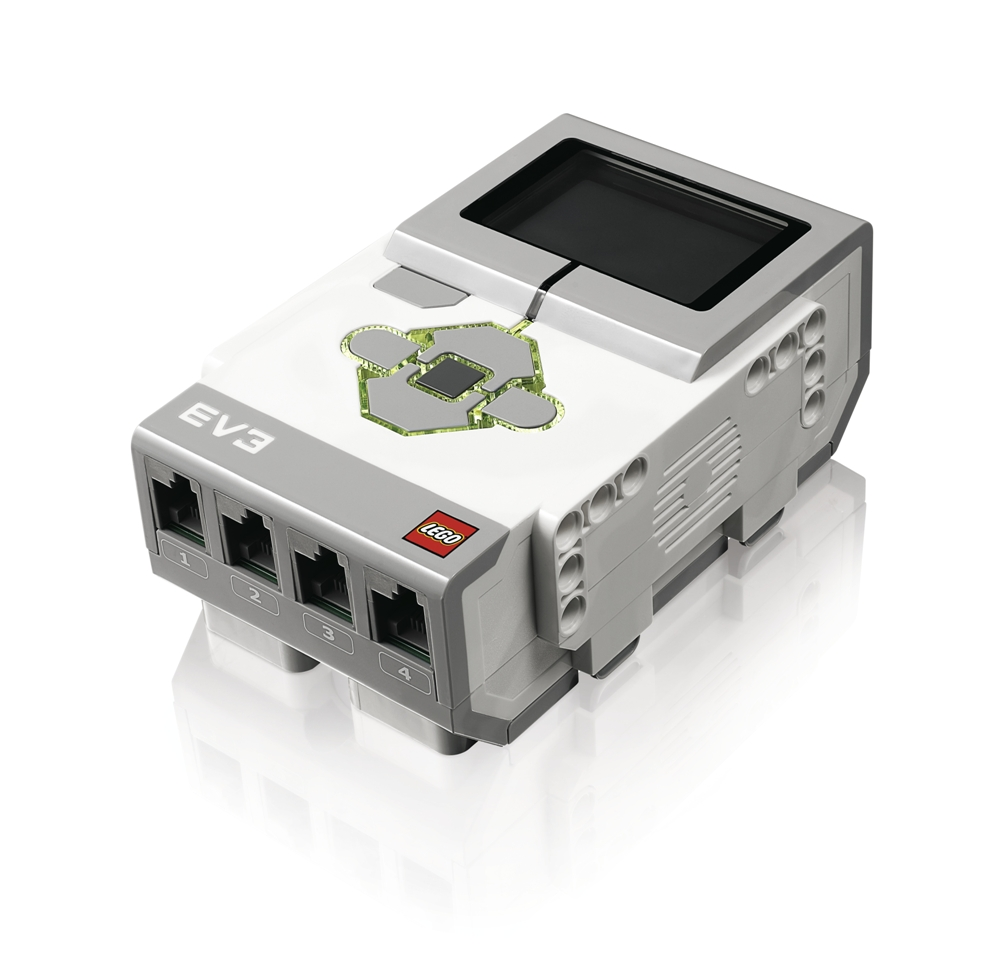
\includegraphics[width=330px]{images/lego-mindstorms-ev3_brick.jpg}
	\caption[\legoEV{ Brick}]{\legoEV{ \brick}\protect\footnotemark}
	\label{fig:lego-mindstorms-ev3_brick}
\end{figure}

\footnotetext{Zdroj: \url{http://hackeducation.com/2015/04/10/mindstorms}} 

Nová verze obsahuje také čtečku Micro SD karet, USB host interface a jeden výstupní port pro motory navíc (celkem 4~porty, NXT jen 3~porty) \cite{legoBotBench_comparing-EV3-and-NXT}. 

Slot na SD karty umožňuje rozšířit paměť pro programy, ale lze jej hlavně využít pro spouštění alternativních operačních systémů. 

Díky USB host interfacu lze k EV3 připojovat různé periferie, pro které je v systému a vývojovém prostředí připravená obsluha.
Lze tak připojit Wifi modul, klávesnici nebo myš. 
Zároveň můžete přes USB kabel spojit až čtyři EV3 \brick{\it y} a ovládat je jedním programem (z jednoho hlavního \brick{\it u}).

\begin{figure}[h]
	\centering
	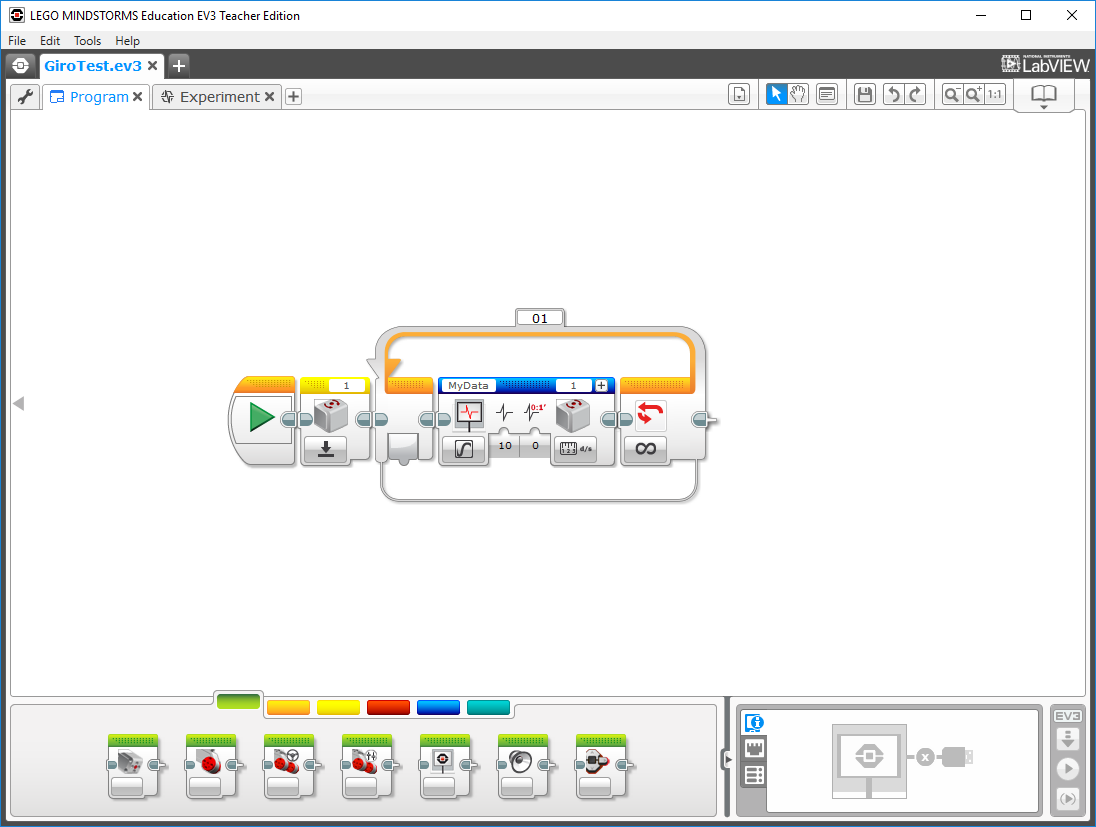
\includegraphics[width=\textwidth]{images/lego-mindstorms-ev3_dev-soft.png}
	\caption[\legoM{ }Education EV3 Software -- vývojové prostředí]{\legoM{ }Education EV3 Software -- vývojové prostředí}
	\label{fig:lego-mindstorms-ev3_dev-soft}
\end{figure}

Programovací prostředí pro EV3 je znovu postaveno na \labview{ } a ačkoliv se design v porovnání s prostředím pro NXT výrazně změnil (můžete porovnat obrázky \ref{fig:lego-mindstorms-nxt-g} a \ref{fig:lego-mindstorms-ev3_dev-soft}) neměli by mít uživatelé NXT s přechodem problém. 
Nové prostředí zvládne naprogramovat jak EV3, tak NXT \brick{}.

V rámci alternativních platforem máme opět velký výběr \cite{legoMindstormsWikipedia_programming-languages}. 
Vhledem k nutnosti používání operačního systému je většinou pro dané prostředí potřeba nahrát konkrétní systém na SD kartu a spustit \brick{ }s touto kartou.

Jednotlivé alternativní platformy budou podrobněji probrány v následující kapitole.
